% -*- coding: utf-8; -*-

\chapter{Pesquisas Realizadas}
\label{cha:Pesquisas Realizadas}


Nesse capítulo serão abordadas todas as pesquisas realizadas para a confecção dessa tese. Os tópicos variam desde temas mais técnicos explorando diferentes tipos de redes neurais e otimizadores, até assuntos mais voltados para a área médica.




\section{Pneumonia}


A pneumonia é uma infecção que inflama os sacos de ar em um ou ambos os pulmões, onde esses sacos podem se encher de líquido ou pus, provocando tosse com pus ou muco, febre, calafrios e dificuldade para respirar, podendo ser melhor representado na imagem \ref{pic:pneumonia}. A condição pode ser causada por uma variedade de organismos, incluindo bactérias, vírus e fungos. A gravidade da pneumonia pode variar de leve a grave, sendo mais perigosa para bebês e crianças pequenas, pessoas com mais de 65 anos e pessoas com problemas de saúde ou sistemas imunológicos enfraquecidos \cite{WHO2023Pneumonia}. Podemos confirmar esses detalhes também na imagem \ref{pic:stats_pneumonia}, onde observamos que em todas as condições as pessoas mais afetas por pneumonia são idosas. Essa imagem retrata um estudo feito da incidência de casos de pneumonia nos EUA dos anos de 2007 até 2010 \cite{doi:10.2147/COPD.S140378}.

\begin{figure}[!ht]
    \begin{center}
    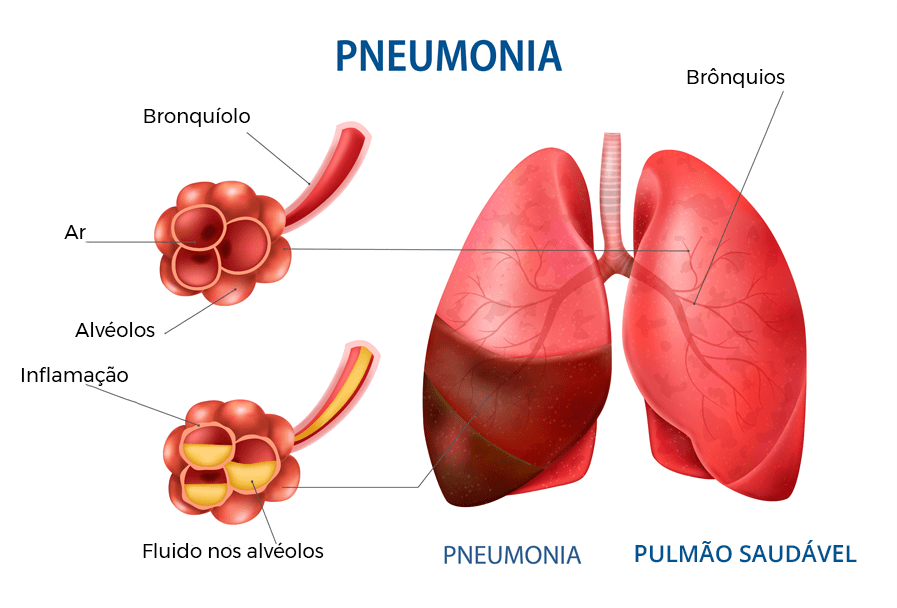
\includegraphics[width=300pt]{pictures/pneumonia -2.png}
    \caption{Pneumonia afetando um pulmão}
    \label{pic:pneumonia}
    \end{center}
\end{figure}

\begin{figure}[!ht]
    \begin{center}
    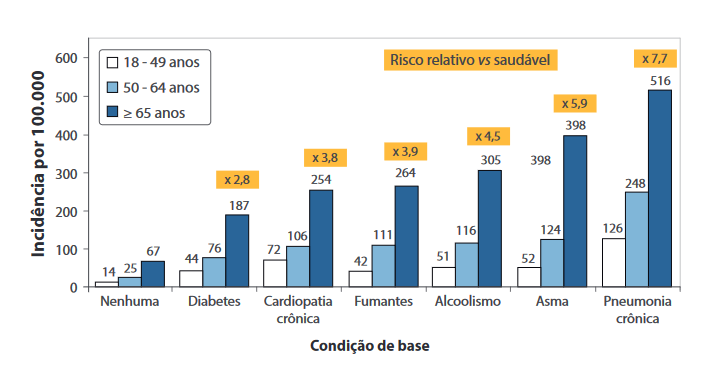
\includegraphics[width=350pt]{pictures/incidencia.png}
    \caption{Incidência de pneumonia em adultos }
    \label{pic:stats_pneumonia}
    \end{center}
\end{figure}




No Brasil, o Sistema Único de Saúde (SUS) registra anualmente mais de 600 mil internações por Pneumonia Adquirida na Comunidade (PAC) e Influenza. De janeiro a agosto de 2022, houve 44.523 mortes por pneumonia no país, um aumento significativo em relação ao mesmo período do ano anterior, que teve 31.027 óbitos. \cite{bvsmsDiaMundialPneumonia}

Em um contexto global, em 2019, a pneumonia foi responsável pela morte de cerca de 2,5 milhões de pessoas. Notavelmente, quase um terço dessas vítimas eram crianças com menos de 5 anos, fazendo da pneumonia a principal causa de morte para crianças nessa faixa etária . Apesar de ainda muitas crianças morrerem devido à pneumonia hoje, desde 1990 houve uma redução de mais de três vezes nas taxas de mortalidade infantil devido à doença em todo o mundo.\cite{OurWorldInDataPneumonia} Em 2019, a pneumonia resultou na morte de 740.180 crianças com menos de cinco anos, correspondendo a 14\% das mortes totais nessa faixa etária e a 22\% das mortes entre crianças de um a cinco anos, impactando famílias globalmente \cite{WHO2023Pneumonia}. 

A pneumonia bacteriana, que é a mais comum, é frequentemente causada pela bactéria \textit{Streptococcus pneumoniae}, embora outras bactérias como \textit{Mycoplasma pneumoniae} e \textit{Chlamydophila pneumoniae} também possam ser responsáveis. A pneumonia viral, por outro lado, é uma causa comum de pneumonia em crianças, com vírus respiratórios sendo os culpados frequentes. A pneumonia fúngica pode ocorrer em pessoas com sistemas imunológicos enfraquecidos \cite{WHO2023Pneumonia}.


Os sintomas da pneumonia podem variar, mas geralmente incluem tosse produtiva, febre, calafrios, fadiga, sudorese, dor no peito, confusão (em pessoas idosas) e falta de ar. O diagnóstico é geralmente feito com base nos sintomas e confirmado através de um exame físico, radiografia de tórax e, possivelmente, exames de sangue e culturas de escarro \cite{WHO2023Pneumonia}.

O tratamento para pneumonia depende da causa. A pneumonia bacteriana é geralmente tratada com antibióticos, enquanto a pneumonia viral pode ser tratada com antivirais. É também importante descansar, manter-se hidratado e tomar medicamentos para aliviar os sintomas. Para prevenção, existem vacinas como a vacina pneumocócica e a vacina contra a gripe, e medidas como lavar as mãos regularmente e evitar contato com pessoas doentes podem ser eficazes \cite{WHO2023Pneumonia}.

As complicações da pneumonia podem ser graves, podendo incluir infecção bacteriana no sangue (sepse), acúmulo de líquido e pus no espaço ao redor do pulmão (empema), e insuficiência respiratória. Indivíduos com sistemas imunológicos enfraquecidos, doenças crônicas, ou que estão em certos grupos etários (como crianças muito pequenas ou idosos) estão em maior risco de desenvolver pneumonia \cite{pneumoniaSymptoms}.  



\section{Redes Neurais}

Redes neurais é uma abordagem computacional ao processamento de informação, similiar ao sistema de nervoso dos seres humanos, especialmente o cérebro. Ela é uma sub-área de aprendizado de máquina, chamado de aprendizado profundo (\textit{deep learning}) capaz de realizar operações mais complexas e que necessitem de um poder computacional maior.

Sua unidade fundamental é chamada de neurônio, sendo apenas uma simplificação matemática do neurônio biológico. 

\begin{figure}[!ht]
    \begin{center}
    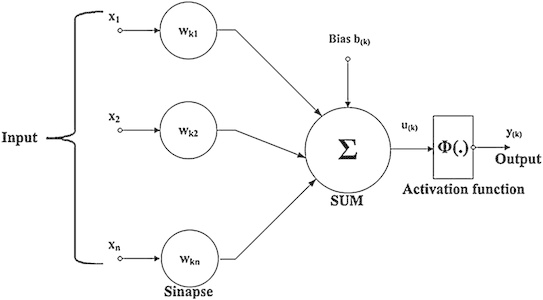
\includegraphics[width=350pt]{pictures/neuronio-matematico.png}
    \caption{Neurônio Matemático}
    \label{pic:neuronio}
    \end{center}
\end{figure}


Como ilustrado na figura \ref{pic:neuronio}, num primeiro momento, as informações são recebidas pelo neurônio em termos matemáticos (representados por $x_1, x_2, ... x_n$), ou seja, deve representar um valor numérico. Isso acontece porque, em uma rede neural, neurônios são conectados uns aos outros de maneira encadeada, por isso, é interessante manter esse padrão. Cada entrada de informação é associada à um peso. Esses pesos são valores númericos ajustáveis (indicados na imagem por $w_{k1}, w_{k2}, ...w_{kn}$ e representam a importância ou influência que uma determinada entrada pode impactar na saída do neurônio. Vale ressaltar que esses pesos inicialmente são definidos aleatoriamente e logo após ajustados durante o treinamento da rede \cite{GoodfellowBengioCourville2016}, \cite{Watt2016MachineLearning}.

\newpage

Recebendo essas entradas, o neurônio multiplica cada uma pelo seu respectivo peso e, em seguida, soma todos os produtos encontrados. Isso é chamado de função de soma, sendo representada na imagem pela letra grega ''$\sum$''. Normalmente esse processo de soma é representado matematicamente por um produto escalar, de um vetor de entradas $X$ por um vetor de pesos $W$.

$$
Soma = w_1 \times x_1 + w_2 \times x_2 + ... + w_n \times x_n
$$

Uma passo importante antes de calcular a soma ponderada é adicionar uma constante chamada de Viés (\textit{Bias}, representado como $b_{(k)}$ na imagem). O viés permite ajustar a saída do neurônio junto com os pesos, proporcionando um grau de liberdade adicional à rede neural. Podemos entender ele como uma maneira de ajustar a ''sensibilidade'' do neurônio. Após essa ''correção'' do viés, na soma ponderada, seu resultado é passado por uma função de ativação $\Phi(.)$, que introduz uma não-linearidade, permitindo que a rede neural modele operações mais complexas. As funções mais utilizadas são: \textbf{Sigmóide} (\ref{subfig:pictures/sigmoid.png}), \textbf{ReLU} (\ref{subfig:pictures/relu_func.png}), \textbf{Tangente Hiperbólica} (\ref{subfig:pictures/tanh.png}), \textbf{Softmax} (sendo frequentemente usada na camada de saída de problemas de classficação) e entre outros \cite{GoodfellowBengioCourville2016}, \cite{Watt2016MachineLearning}. 


\subimages{Funções de ativação}{45}
{
 \subimage[Sigmóide]{.35}{pictures/sigmoid.png}
 \subimage[ReLU]{.35}{pictures/relu_func.png}\\
 \subimage[Tangente Hiperbólica]{.35}{pictures/tanh.png} 
}


Por fim, o valor produzido pela função de ativação se torna a saída do neurônio. Como dito anteriormente, esse valor pode ser passado para outros neurônios, em sequência, ou até mesmo ser a saída definitiva da rede.

Para termos uma visão mais geral, podemos entender o processo de ativação da seguinte maneira:

\begin{enumerate}
    \item O neurônio recebe várias entradas
    \item Cada entrada é mutiplicada por seu respectivo peso
    \item Os produtos são somados junto ao \textit{Bias}
    \item A soma resultante passa por uma função de ativação para produzir a saída
\end{enumerate}

O objetivo do treinamento de uma rede neural é ajustar os pesos e vieses para que eles se adequem ao conjunto de dados fornecidos gerando uma saída muito próxima da desejada. Esses ajustes podem ser feitos utilizandos técnicas como o gradiente descente e a propagação reversa (\textit{backpropagation}) \cite{58337} \cite{Watt2016MachineLearning}.   



\section{Convolutional Neural Networks}

AS CNNs, também conhecidas como Redes Neurais Convolucionais, são uma categoria de redes neurais que se mostrou particularmente eficaz para tarefas de processamento de imagem. As CNNs são insipiradas pela visão biológica e foram projetadas para reconhecer padrões diretamente dos pixels de imagens com mínimo pré-processamento. A operação central das CNNs é a convolução. Ao invés de conectar totalmente todos os neurônios da camada anterior, um neurônio está conectado apenas a um pequeno patch localizado na camada anterior, através de um objeto matemático chamado de filtro ou \textit{kernel}. Um Kernel é uma matriz pequena, geralmente de tamanho $n \times n$, onde $n$ é um número ímpar como 3, 5 ou 7. Este kernel é ''deslizado'' ao longo da imagem para produzir um novo mapa de características.\cite{GoodfellowBengioCourville2016} Em cada ''deslizamento'' ocorre uma operação de convolução, que pode ser definida da seguinte maneira: 

Sejam $f(\tau)$ e $k(\tau)$ duas funções de domínio em $\mathbb{R}$, uma operação de convolução entre ambas pode ser escrita como:

$$
f \ast k = \int_{- \infty}^{\infty} f(\tau)k(t - \tau) \,dt 
$$

Numa camada convolucional, podemos generalizar a expressão de ''deslizamento'' do \textit{kernel} $k$ por uma imagem $I$ de tamanho $m \times n$, da seguinte forma:

$$
k \ast I = Z(i,j) = \sum_{m} \sum_{n}{k(m,n) I(i - m, j - n)}
$$

É importante ressaltar também que existem outras configurações que podemos alterar no \textit{kernel} para torná-lo mais preciso de modificável. Umas da alterações que podemos fazer é em relação a quantidade de pixels que ele se move de cada vez, ou melhor, a quantidade de pixels que é desconsiderada em cada turno. Essa disposição é chamada de \textit{stride} e está representada na imagem \ref{pic:stride} \cite{GoodfellowBengioCourville2016}. 


\begin{figure}[!ht]
    \begin{center}
    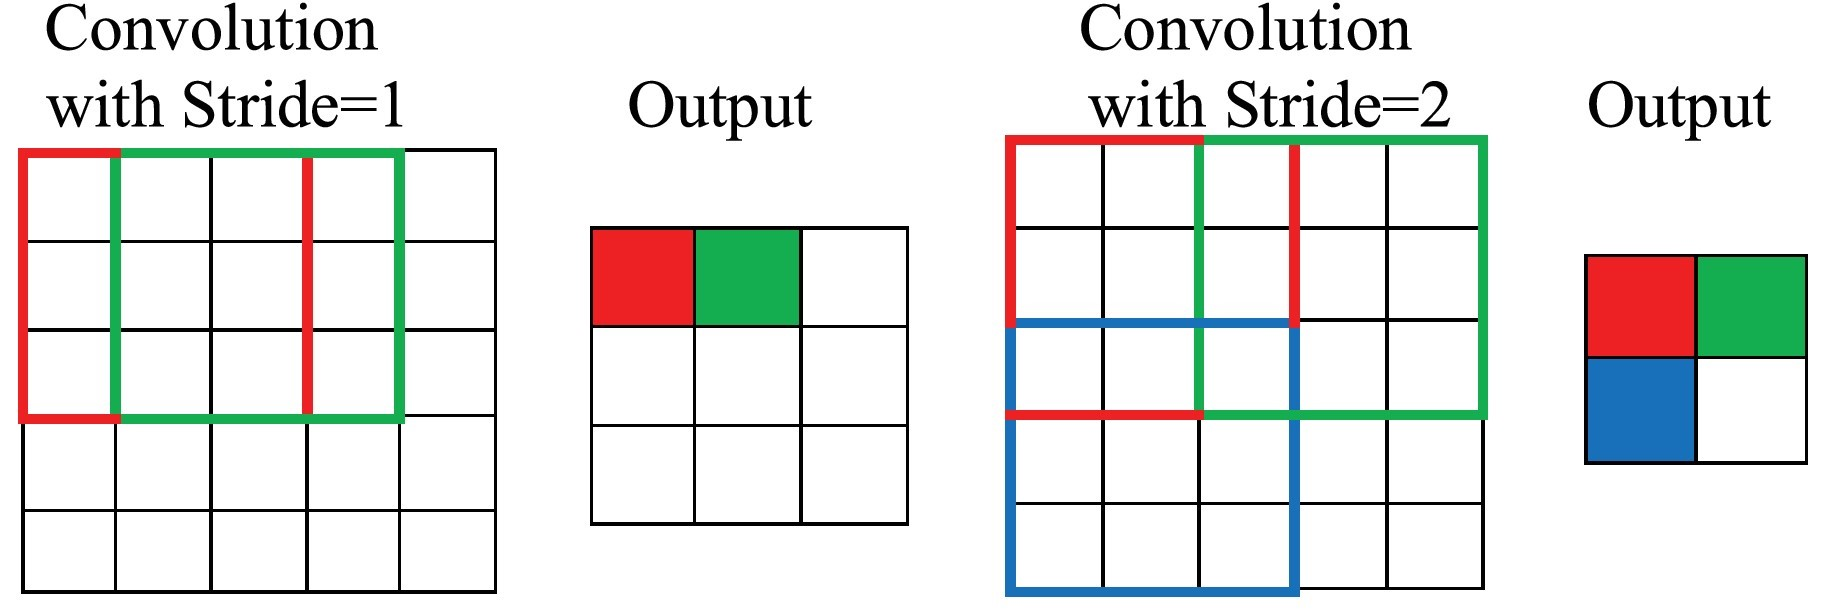
\includegraphics[width=350pt]{pictures/stride.jpg}
    \caption{Exemplo de stride}
    \label{pic:stride}
    \end{center}
\end{figure}


Outro conceito importante é o \textit{padding}, representado na imagem \ref{pic:padding}, que consiste em adicionar zeros ao entorno da imagem, ou do mapa de característica para controlar a dimensão espacial do resultado, usado frequentemente para manter a mesma dimensão espacial após a convolução \cite{GoodfellowBengioCourville2016}.


\begin{figure}[!ht]
    \begin{center}
    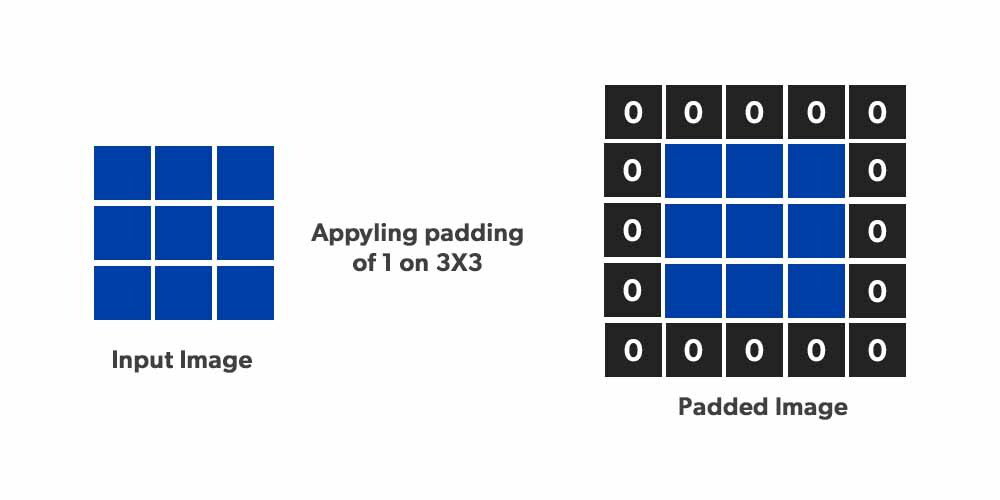
\includegraphics[width=350pt]{pictures/padding.jpg}
    \caption{Exemplo de padding}
    \label{pic:padding}
    \end{center}
\end{figure}


Um outro detalhe importante que precisa ser mencionado é sobre o canal de cores. Naturalmente, essa operações que foram descritas anteriormente são realizadas em apenas 1 dos canais da imagem, ou seja, se quisermos aplicar a metodologia apresentada, devemos repetir o processo para todos os canais \textbf{\textit{Red}}, \textbf{\textit{Green}} e \textbf{\textit{Blue}} \cite{Watt2016MachineLearning}.



Após passar pela camada convolucional, sua saída é passada por uma função de ativação, como mostrado na seção de \textbf{Redes Neurais}. Nesse caso, normalmente é utilizada a função ReLU (\textit{Rectified Linear Unit}) devido a sua eficácia \cite{Watt2016MachineLearning}.


\begin{figure}[!ht]
    \begin{center}
    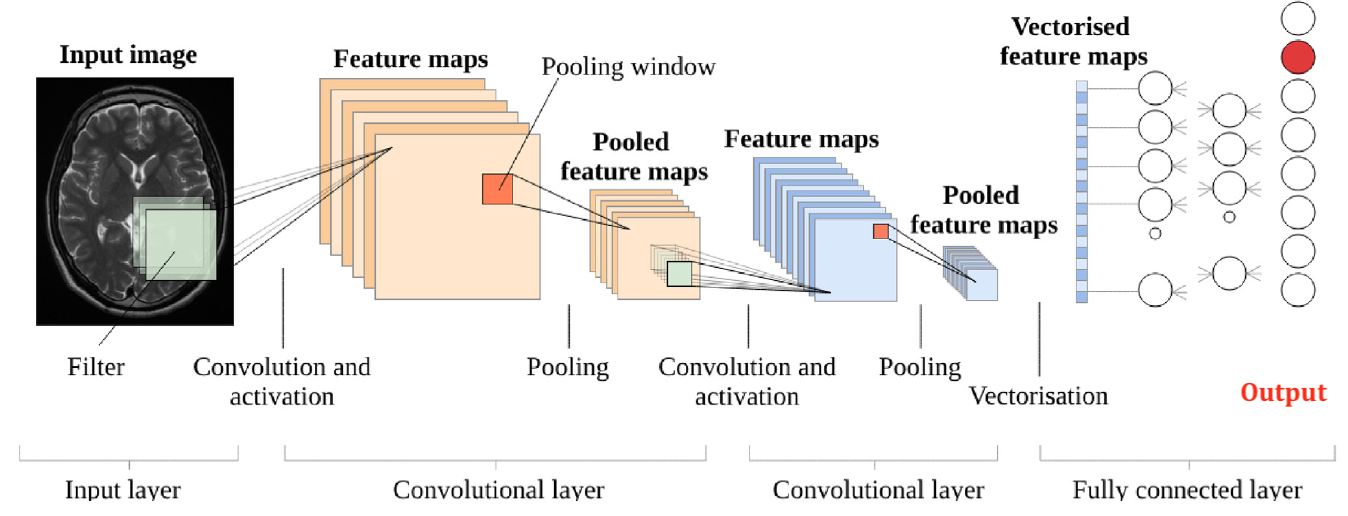
\includegraphics[width=350pt]{pictures/cnn_example_brain.png}
    \caption{\href{https://mriquestions.com/deep-network-types.html}{Visão completa de uma CNN}}
    \label{pic:cnn_complete}
    \end{center}
\end{figure}

Na imagem \ref{pic:cnn_complete} observamos todos os estágios para a criação de uma CNN, desde sua camada de \textit{input} até sua sáida. Percebemos também a presença de todas as camadas comentadas no texto, como as de convolução, \textit{polling} e a camada totalmente conectada.

\section{ResNet50}

A ResNet50 é uma variante da arquitetura de rede neural conhecida como Residual Network (ResNet), que foi uma das contribuições mais significativas no campo da visão computacional, particularmente no contexto de reconhecimento de imagens profundas. Desenvolvida por Kaiming He, Xiangyu Zhang, Shaoqing Ren e Jian Sun da Microsoft Research, estabelecendo um novo estado da arte para a classificação de imagens \cite{He2015}.

O principal problema que as conexões residuais visam resolver é o do "desaparecimento do gradiente", que é um desafio comum ao treinar redes neurais profundas. À medida que a rede se aprofunda, os gradientes (que são essenciais para a atualização dos pesos durante o treinamento) podem se tornar tão pequenos que não têm efeito perceptível, tornando a rede difícil ou impossível de treinar. As conexões residuais permitem que o sinal de gradiente seja diretamente propagado para camadas anteriores sem passar por todas as transformações de camadas intermediárias. Isso é feito adicionando a saída de uma camada anterior à saída de uma camada mais avançada, efetivamente permitindo que a rede aprenda a função de identidade se necessário. Isso significa que, em vez de aprender uma transformação direta, as camadas estão aprendendo um resíduo \cite{He2015}.

A ResNet50 é estruturada em quatro estágios principais, contendo uma série de blocos residuais, com o número de blocos em cada estágio sendo 3, 4, 6 e 3, respectivamente. À medida que a rede progride através dos estágios, o tamanho das características é reduzido e o número de filtros é aumentado para manter a carga computacional gerenciável \cite{Sharma2022Enhanced}.

Após todos os blocos residuais, a rede aplica uma camada de average pooling para condensar as características espaciais em um único vetor por característica. Isso é seguido por uma camada totalmente conectada que mapeia as características para o número desejado de classes e uma camada softmax para calcular as probabilidades de classificação \cite{Sharma2022Enhanced}.

Durante o treinamento, as conexões residuais facilitam a otimização da rede, mesmo com sua profundidade significativa. A ResNet50 pode ser treinada a partir do zero ou usada como uma rede pré-treinada em grandes conjuntos de dados, como o ImageNet, e ajustada para tarefas específicas através da transferência de aprendizado.


\begin{figure}[!ht]
    \begin{center}
    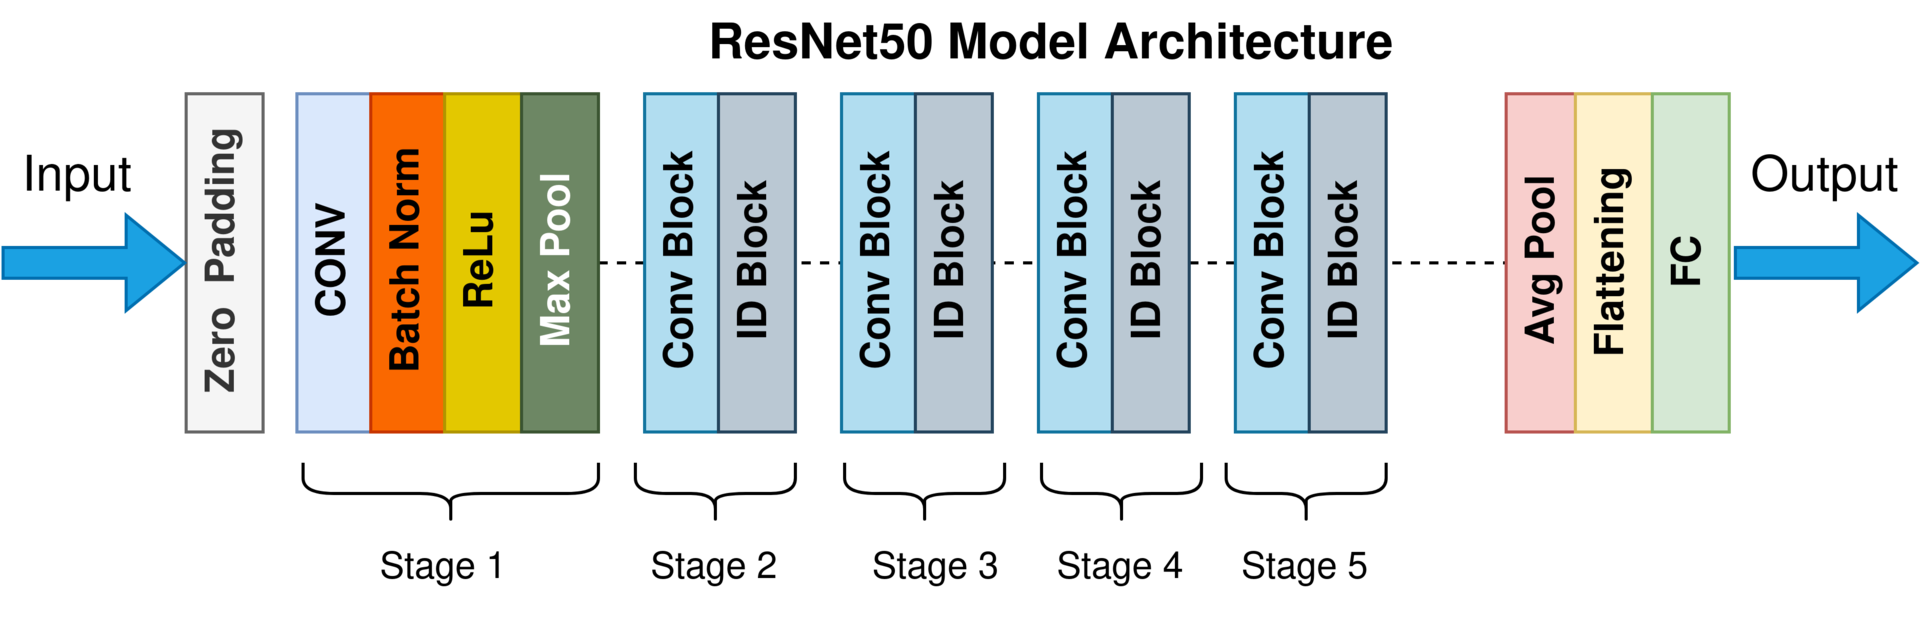
\includegraphics[width=350pt]{pictures/ResNet50.png}
    \caption{Arquitetura da ResNet50}
    \label{pic:resnet50}
    \end{center}
\end{figure}


Como representado na arquitetura da ResNet na imagem \ref{pic:resnet50}, a rede começa com uma única camada de convolução seguida por uma camada de max pooling, depois segue para uma série de blocos residuais e termina com uma camada de average pooling, uma camada totalmente conectada e uma função de ativação, como por exemplo a softmax, para tarefas de classificação.

A ResNet50, devido à sua profundidade e eficiência, tornou-se uma escolha popular para muitas aplicações de visão computacional, incluindo reconhecimento de objetos, detecção de objetos e segmentação semântica. Ela também é frequentemente usada como uma rede pré-treinada para transferência de aprendizado, onde uma rede treinada em um grande conjunto de dados (como o ImageNet) é adaptada para uma tarefa específica com um conjunto de dados menor \cite{Sharma2022Enhanced}.

O sucesso da ResNet e suas variantes inspirou muitas outras arquiteturas de redes neurais e continua a ser uma área ativa de pesquisa e aplicação. A capacidade de treinar redes profundas sem o problema do desaparecimento do gradiente abriu novas possibilidades para o design de arquiteturas de rede neural e ajudou a avançar o campo da inteligência artificial. Podemos entender mais até sobre o modelo e sua forma como foi construído no reposítório oficial da biblioteca TensorFlow, utilizada nessa tese, acesse \href{https://github.com/tensorflow/tpu/tree/master/models/experimental/resnet50_keras}{\textbf{Tensorflow: ResNet50}}


\section{InceptionV3}

Outro modelo de Rede Neural mundialmente utilizado é a InceptionV3. Ele foi introduzido pela primeira vez em 2014 por pesquisadores da Google na sua primeira versão (InceptionV1 ou GoogLeNet), após ter ganhado o desafio de classficação de imagem \textit{ImageNet Large Scale Visual Recognition Challenge} (\textbf{ILSVRC}) \cite{Szegedy2015RethinkingTI}. 

O modelo Inception v1 introduziu o conceito de módulos Inception. Eles foram criados com o objetivo de tornar as redes neurais convolucionais mais adaptáveis e capazes de extrair informações de uma vasta gama de entradas de imagem. A funcionalidade desses módulos se baseia em realizar várias operações de convolução simultaneamente, cada uma com filtros de tamanhos distintos, como 1x1, 3x3 e 5x5. Essa variedade permite que a rede detecte desde os detalhes mais sutis até as características mais amplas e abstratas das imagens. Em paralelo às convoluções, os módulos também executam operações de pooling, geralmente do tipo max pooling, que contribuem para a redução da dimensionalidade dos dados e ajudam a rede a se tornar invariante a pequenas mudanças e deslocamentos na imagem. Após realizar as convoluções e o pooling, a rede combina as saídas de todas essas operações paralelas, concatenando-as. Essa concatenação é feita ao longo do eixo do canal, garantindo que a riqueza de informações capturadas em cada processo seja mantida e transmitida adiante na rede \cite{7298594}.

Para evitar um crescimento exponencial no número de cálculos necessários, devido ao aumento das dimensões, os módulos Inception aplicam uma técnica de redução de dimensão. Isso é feito através do uso de convoluções 1x1 antes de aplicar filtros maiores, o que diminui a profundidade do volume de entrada sem perder informações essenciais. Com essa abordagem no modelo, podemos garatir que a rede neural mantenha sua eficiência computacional, mesmo enquanto processo grandes quantidades de dados \cite{7298594}.

Após as inovações da sua primeira versão, foi uma lançada uma V2 que trouxe uma melhoria na sua arquitetura original, incluindo otimizações para reduzir mais ainda o consumo operacional. Uma das melhorias inseridas foi a adição da \textit{batch normalization}, que por consequência, acelerou o treinamento do modelo \cite{PapersWithCode_InceptionV2}.

 A Inception v3 trouxe avanços notáveis em relação às suas versões antecessoras, mantendo as otimizações da Inception v2 e adicionando novas melhorias. A arquitetura, como representada na imagem \ref{pic:inceptionv3}, refinou os módulos Inception com ajustes que padronizam os tamanhos dos filtros de convolução, resultando em uma redução substancial do número de operações computacionais necessárias. Além disso, a Inception v3 substituiu as convoluções de maior dimensão por uma sequência de duas convoluções de 3x3, diminuindo assim o número de parâmetros e o custo computacional envolvido \cite{Szegedy2016RethinkingTI}.

\begin{figure}[!ht]
    \begin{center}
    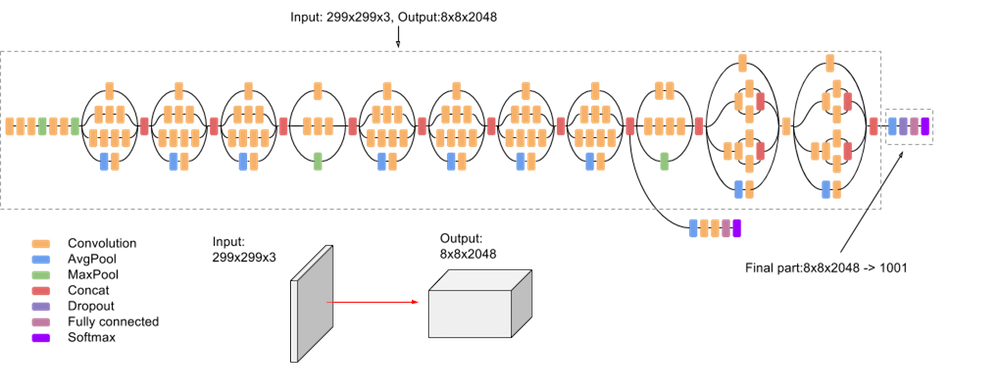
\includegraphics[width=350pt]{pictures/inception.png}
    \caption{Arquitetura da InceptionV3}
    \label{pic:inceptionv3}
    \end{center}
\end{figure}


Como citado anteriormente, a arquitetura também adotou o uso de convoluções assimétricas, empregando uma combinação de convoluções 1xN seguidas por Nx1, uma estratégia eficaz para substituir as convoluções quadradas tradicionais e reduzir ainda mais as demandas computacionais sem comprometer a eficiência na detecção de características. Para fortalecer a capacidade do modelo de generalizar a partir de conjuntos de dados de treinamento, a Inception v3 integrou técnicas de ampliação de dados mais avançadas, aumentando a robustez do modelo ao expô-lo a uma variedade mais ampla de variações de imagem durante o treinamento \cite{7298594}, \cite{Szegedy2016RethinkingTI}. Podemos entender mais até sobre o modelo e sua forma como foi construído no reposítório oficial da biblioteca TensorFlow, utilizada nessa tese, acesse \href{https://github.com/tensorflow/tpu/tree/master/models/experimental/inception}{\textbf{Tensorflow: Inception}}



\section{Otimizador RMSprop}

Algoritmos de otimização como desempenham um papel crucial no treinamento de redes neurais e outros modelos de aprendizado de máquina, pois aceleram a convergência para o mínimo da função de custo, o que é determinante para a avaliação do desempenho do modelo. Essa aceleração resulta em economia de tempo e recursos computacionais. Além disso, esses algoritmos previnem que o modelo fique retido em mínimos locais ou pontos de sela, garantindo assim que as soluções encontradas sejam robustas e representativas das melhores configurações possíveis \cite{Watt2016MachineLearning}. 

A capacidade de ajustar hiperparâmetros como a taxa de aprendizado é outra vantagem significativa, já que alguns algoritmos adaptam esses parâmetros dinamicamente durante o treinamento, potencialmente levando a resultados superiores. Eles são particularmente eficientes em grandes conjuntos de dados, onde calcular o gradiente para todos os exemplos é impraticável, optando por atualizar os parâmetros usando mini-lotes de dados \cite{Watt2016MachineLearning}.

A adaptabilidade desses algoritmos também permite que se ajustem a uma variedade de problemas, especialmente aqueles com superfícies de erro irregulares, suavizando as oscilações e promovendo atualizações mais consistentes. Eles mantêm a estabilidade numérica durante o treinamento, evitando extremos que poderiam resultar em problemas computacionais. Finalmente, ao otimizar a função de custo, contribuem para a capacidade de generalização do modelo, melhorando seu desempenho em dados novos e, portanto, sua utilidade em aplicações do mundo real \cite{Watt2016MachineLearning}.

Um dos algorítmos de otimização utilizado é o RMSProp, abreviação de "\textit{Root Mean Square Propagation}". Ele é um algoritmo de otimização projetado especificamente para treinar redes neurais artificiais (ANNs) e foi proposto por Geoff Hinton durante um curso online sobre Redes Neurais para Aprendizado de Máquina \cite{elshamy2023improving}.

Este algoritmo é uma adaptação do \textit{Stochastic Gradient Descent} (SGD) e faz parte dos métodos de taxa de aprendizagem adaptativa. O principal objetivo do RMSProp é ajustar de forma mais eficaz a taxa de aprendizagem durante o processo de treinamento. Para fazer isso, mantém uma média móvel (descontada) do quadrado dos gradientes e usa essa média para normalizar o gradiente ao atualizar os pesos da rede. Ou seja, ajusta a taxa de aprendizagem para cada parâmetro individualmente, em vez de ter uma taxa de aprendizagem fixa para todos os parâmetros \cite{elshamy2023improving}. Podemos escrever os cálculos de atualização da seguinte forma:

$$
E [g^2]_t = \beta E[g^2]_{t-1} + (1 - \beta)(\frac{\partial C}{\partial w})^2 
$$
$$
w_t = w_{t-1} - \frac{\eta}{\sqrt{E[g^2]_t}}\frac{\partial C}{ \partial w}
$$


Onde, $E[g]$ é a média móvel dos quadrados do gradientes, $\frac{\partial C}{\partial w}$ é o gradiente da função de custo com o respectivo peso ($w$); A constante $\eta$ é a taxa de aprendizado e $\beta$ é o parâmetro da média móvel, sendo normalmente utilizado como $0.9$ no seu valor.


\section{Otimizador Adam}

O otimizador Adam, abreviação de "\textit{Adaptive Moment Estimation}", é um algoritmo para otimização que é usado amplamente no treinamento de redes neurais e outras aplicações de aprendizado de máquina. Ele foi introduzido por Kingma e Ba em 2014 e é particularmente eficiente em casos com grandes volumes de dados e parâmetros, como mostram problemas envolvendo imagem \cite{Watt2016MachineLearning}.

Adam combina ideias do "\textit{momentum}" e do "RMSprop". No "\textit{momentum}", utiliza-se a média exponencialmente ponderada dos gradientes para acelerar o gradiente descendente. Esta técnica ajuda o algoritmo a acelerar em direções consistentes, o que auxilia na convergência mais rápida para mínimos. O RMSprop, por outro lado, adapta a taxa de aprendizado para cada parâmetro ao calcular uma média móvel exponencial dos quadrados dos gradientes. Isso permite ajustes mais finos do aprendizado, evitando passos demasiadamente grandes ou pequenos que poderiam prejudicar a convergência \cite{gess2023convergence}.

O otimizador Adam, portanto, herda as vantagens de ambos os métodos, oferecendo uma abordagem que consegue lidar bem com a variação nos gradientes e a escala dos dados. Isso é feito mantendo estimativas separadas dos primeiros momentos (o equivalente ao momentum) e dos segundos momentos (o equivalente ao RMSprop) dos gradientes \cite{gess2023convergence}.

O aspecto matemático do Adam envolve o cálculo das médias móveis exponencialmente ponderadas dos gradientes e dos quadrados dos gradientes. Entretanto, como essas médias são inicializadas como zero, o otimizador faz uma "correção de viés" para ajustar e escalar as médias móveis, garantindo que elas sejam imparciais. Intuitivamente, o Adam ajusta a descida do gradiente após cada iteração para mantê-la sob controle e imparcial durante todo o processo de otimização \cite{Watt2016MachineLearning}.

Em termos de desempenho, o Adam é conhecido por superar muitos outros otimizadores, proporcionando um treinamento eficiente e eficaz, com menor custo computacional e melhor desempenho em muitos cenários. O ajuste fino que o Adam proporciona, ao controlar a taxa de aprendizado de maneira adaptativa, permite que ele navegue eficientemente através de paisagens complexas de otimização, alcançando bons mínimos em tempo hábil e com estabilidade \cite{gess2023convergence}.


\begin{figure}[!ht]
    \begin{center}
    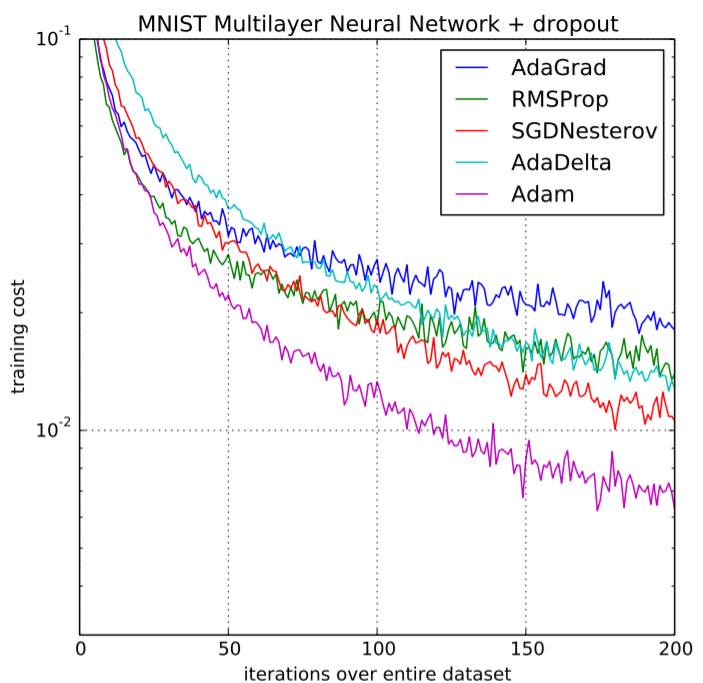
\includegraphics[width=250pt]{pictures/performance.png}
    \caption{Performance entre otimizadores}
    \label{pic:performance}
    \end{center}
\end{figure}


A imagem \ref{pic:performance}, mostra um comparativo entre diversos otimizadores aplicados à tarefa de classificar imagens do conjunto de dados \textbf{MNIST}, torna-se evidente que, apesar de todos visarem a minimização do erro, o Adam sobressai significativamente em termos de desempenho ao longo das iterações. Em contrapartida, o RMSProp, mencionado previamente, exibe um desempenho consistente, mas não extraordinário, situando-se em um patamar intermediário em relação aos demais otimizadores analisados.



%https://mriquestions.com/deep-network-types.html
